
%% This LaTeX template is based on the following example file included in the ieeetran
%% package:
%% bare_conf.tex 
%% V1.2
%% 2002/11/18
%% by Michael Shell
%% mshell@ece.gatech.edu
%% (requires IEEEtran.cls version 1.6b or later) with an IEEE conference paper.


% Note that the a4paper option is mainly intended so that authors in
% countries using A4 can easily print to A4 and see how their papers will
% look in print. Authors are encouraged to use U.S. letter paper when 
% submitting to IEEE. Use the testflow package mentioned above to verify
% correct handling of both paper sizes by the author's LaTeX system.
%
% Also note that the "draftcls" or "draftclsnofoot", not "draft", option
% should be used if it is desired that the figures are to be displayed in
% draft mode.
%
% This paper can be formatted using the peerreviewca
% (instead of conference) mode.
\documentclass[conference, a4paper]{IEEEtran-modified}
% If the IEEEtran.cls has not been installed into the LaTeX system files, 
% manually specify the path to it:
% \documentclass[conference]{../sty/IEEEtran} 

\IEEEoverridecommandlockouts

% some very useful LaTeX packages include:

\usepackage{cite}       % Written by Donald Arseneau
                        % V1.6 and later of IEEEtran pre-defines the format
                        % of the cite.sty package \cite{} output to follow
                        % that of IEEE. Loading the cite package will
                        % result in citation numbers being automatically
                        % sorted and properly "ranged". i.e.,
                        % [1], [9], [2], [7], [5], [6]
                        % (without using cite.sty)
                        % will become:
                        % [1], [2], [5]--[7], [9] (using cite.sty)
                        % cite.sty's \cite will automatically add leading
                        % space, if needed. Use cite.sty's noadjust option
                        % (cite.sty V3.8 and later) if you want to turn this
                        % off. cite.sty is already installed on most LaTeX
                        % systems. The latest version can be obtained at:
                        % http://www.ctan.org/tex-archive/macros/latex/contrib/supported/cite/

%\usepackage{graphicx}  % Written by David Carlisle and Sebastian Rahtz
                        % Required if you want graphics, photos, etc.
                        % graphicx.sty is already installed on most LaTeX
                        % systems. The latest version and documentation can
                        % be obtained at:
                        % http://www.ctan.org/tex-archive/macros/latex/required/graphics/
                        % Another good source of documentation is "Using
                        % Imported Graphics in LaTeX2e" by Keith Reckdahl
                        % which can be found as esplatex.ps and epslatex.pdf
                        % at: http://www.ctan.org/tex-archive/info/
% NOTE: for dual use with latex and pdflatex, instead load graphicx like:
\ifx\pdfoutput\undefined
	\usepackage{graphicx}
\else
	\usepackage[pdftex]{graphicx}
\fi

% However, be warned that pdflatex will require graphics to be in PDF
% (not EPS) format and will preclude the use of PostScript based LaTeX
% packages such as psfrag.sty and pstricks.sty. IEEE conferences typically
% allow PDF graphics (and hence pdfLaTeX). However, IEEE journals do not
% (yet) allow image formats other than EPS or TIFF. Therefore, authors of
% journal papers should use traditional LaTeX with EPS graphics.
%
% The path(s) to the graphics files can also be declared: e.g.,
% \graphicspath{{../eps/}{../ps/}}
% if the graphics files are not located in the same directory as the
% .tex file. This can be done in each branch of the conditional above
% (after graphicx is loaded) to handle the EPS and PDF cases separately.
% In this way, full path information will not have to be specified in
% each \includegraphics command.
%
% Note that, when switching from latex to pdflatex and vice-versa, the new
% compiler will have to be run twice to clear some warnings.
\graphicspath{{figures/}}


%\usepackage{psfrag}    % Written by Craig Barratt, Michael C. Grant,
                        % and David Carlisle
                        % This package allows you to substitute LaTeX
                        % commands for text in imported EPS graphic files.
                        % In this way, LaTeX symbols can be placed into
                        % graphics that have been generated by other
                        % applications. You must use latex->dvips->ps2pdf
                        % workflow (not direct pdf output from pdflatex) if
                        % you wish to use this capability because it works
                        % via some PostScript tricks. Alternatively, the
                        % graphics could be processed as separate files via
                        % psfrag and dvips, then converted to PDF for
                        % inclusion in the main file which uses pdflatex.
                        % Docs are in "The PSfrag System" by Michael C. Grant
                        % and David Carlisle. There is also some information 
                        % about using psfrag in "Using Imported Graphics in
                        % LaTeX2e" by Keith Reckdahl which documents the
                        % graphicx package (see above). The psfrag package
                        % and documentation can be obtained at:
                        % http://www.ctan.org/tex-archive/macros/latex/contrib/supported/psfrag/

%\usepackage{subfigure} % Written by Steven Douglas Cochran
                        % This package makes it easy to put subfigures
                        % in your figures. i.e., "figure 1a and 1b"
                        % Docs are in "Using Imported Graphics in LaTeX2e"
                        % by Keith Reckdahl which also documents the graphicx
                        % package (see above). subfigure.sty is already
                        % installed on most LaTeX systems. The latest version
                        % and documentation can be obtained at:
                        % http://www.ctan.org/tex-archive/macros/latex/contrib/supported/subfigure/

%\usepackage{url}       % Written by Donald Arseneau
                        % Provides better support for handling and breaking
                        % URLs. url.sty is already installed on most LaTeX
                        % systems. The latest version can be obtained at:
                        % http://www.ctan.org/tex-archive/macros/latex/contrib/other/misc/
                        % Read the url.sty source comments for usage information.

%\usepackage{stfloats}  % Written by Sigitas Tolusis
                        % Gives LaTeX2e the ability to do double column
                        % floats at the bottom of the page as well as the top.
                        % (e.g., "\begin{figure*}[!b]" is not normally
                        % possible in LaTeX2e). This is an invasive package
                        % which rewrites many portions of the LaTeX2e output
                        % routines. It may not work with other packages that
                        % modify the LaTeX2e output routine and/or with other
                        % versions of LaTeX. The latest version and
                        % documentation can be obtained at:
                        % http://www.ctan.org/tex-archive/macros/latex/contrib/supported/sttools/
                        % Documentation is contained in the stfloats.sty
                        % comments as well as in the presfull.pdf file.
                        % Do not use the stfloats baselinefloat ability as
                        % IEEE does not allow \baselineskip to stretch.
                        % Authors submitting work to the IEEE should note
                        % that IEEE rarely uses double column equations and
                        % that authors should try to avoid such use.
                        % Do not be tempted to use the cuted.sty or
                        % midfloat.sty package (by the same author) as IEEE
                        % does not format its papers in such ways.

\usepackage{amsmath}    % From the American Mathematical Society
                        % A popular package that provides many helpful commands
                        % for dealing with mathematics. Note that the AMSmath
                        % package sets \interdisplaylinepenalty to 10000 thus
                        % preventing page breaks from occurring within multiline
                        % equations. Use:
\interdisplaylinepenalty=2500
                        % after loading amsmath to restore such page breaks
                        % as IEEEtran.cls normally does. amsmath.sty is already
                        % installed on most LaTeX systems. The latest version
                        % and documentation can be obtained at:
                        % http://www.ctan.org/tex-archive/macros/latex/required/amslatex/math/



% Other popular packages for formatting tables and equations include:

%\usepackage{array}
% Frank Mittelbach's and David Carlisle's array.sty which improves the
% LaTeX2e array and tabular environments to provide better appearances and
% additional user controls. array.sty is already installed on most systems.
% The latest version and documentation can be obtained at:
% http://www.ctan.org/tex-archive/macros/latex/required/tools/

% Mark Wooding's extremely powerful MDW tools, especially mdwmath.sty and
% mdwtab.sty which are used to format equations and tables, respectively.
% The MDWtools set is already installed on most LaTeX systems. The lastest
% version and documentation is available at:
% http://www.ctan.org/tex-archive/macros/latex/contrib/supported/mdwtools/


% V1.6 of IEEEtran contains the IEEEeqnarray family of commands that can
% be used to generate multiline equations as well as matrices, tables, etc.


% Also of notable interest:

% Scott Pakin's eqparbox package for creating (automatically sized) equal
% width boxes. Available:
% http://www.ctan.org/tex-archive/macros/latex/contrib/supported/eqparbox/



% Notes on hyperref:
% IEEEtran.cls attempts to be compliant with the hyperref package, written
% by Heiko Oberdiek and Sebastian Rahtz, which provides hyperlinks within
% a document as well as an index for PDF files (produced via pdflatex).
% However, it is a tad difficult to properly interface LaTeX classes and
% packages with this (necessarily) complex and invasive package. It is
% recommended that hyperref not be used for work that is to be submitted
% to the IEEE. Users who wish to use hyperref *must* ensure that their
% hyperref version is 6.72u or later *and* IEEEtran.cls is version 1.6b 
% or later. The latest version of hyperref can be obtained at:
%
% http://www.ctan.org/tex-archive/macros/latex/contrib/supported/hyperref/
%
% Also, be aware that cite.sty (as of version 3.9, 11/2001) and hyperref.sty
% (as of version 6.72t, 2002/07/25) do not work optimally together.
% To mediate the differences between these two packages, IEEEtran.cls, as
% of v1.6b, predefines a command that fools hyperref into thinking that
% the natbib package is being used - causing it not to modify the existing
% citation commands, and allowing cite.sty to operate as normal. However,
% as a result, citation numbers will not be hyperlinked. Another side effect
% of this approach is that the natbib.sty package will not properly load
% under IEEEtran.cls. However, current versions of natbib are not capable
% of compressing and sorting citation numbers in IEEE's style - so this
% should not be an issue. If, for some strange reason, the user wants to
% load natbib.sty under IEEEtran.cls, the following code must be placed
% before natbib.sty can be loaded:
%
% \makeatletter
% \let\NAT@parse\undefined
% \makeatother
%
% Hyperref should be loaded differently depending on whether pdflatex
% or traditional latex is being used:
%
%\ifx\pdfoutput\undefined
%\usepackage[hypertex]{hyperref}
%\else
%\usepackage[pdftex,hypertexnames=false]{hyperref}
%\fi
%
% Pdflatex produces superior hyperref results and is the recommended
% compiler for such use.



% *** Do not adjust lengths that control margins, column widths, etc. ***
% *** Do not use packages that alter fonts (such as pslatex).         ***
% There should be no need to do such things with IEEEtran.cls V1.6 and later.

\usepackage[outputdir=build]{minted}
\usepackage{tcolorbox}
\tcbuselibrary{minted,skins}

% Patch to fix https://github.com/T-F-S/tcolorbox/issues/12
\makeatletter
\def\tcb@minted@input@listing#1#2#3#4{%
  \edef\temp@a{#4}%
  \ifx\temp@a\@empty%
  \else%
    \toks@=\expandafter{#4}%
    \edef\tcb@temp{\noexpand\usemintedstyle{\the\toks@}}%
    \tcb@temp%
  \fi%
  \toks@=\expandafter{#1}%
  \edef\tcb@temp{\noexpand\inputminted[\the\toks@]}%
  \IfFileExists{\minted@outputdir#3}%
    {\tcb@temp{#2}{\minted@outputdir#3}}%
    {\tcb@temp{#2}{#3}}%
}
\makeatother

\newtcblisting{myjulia}{%
  listing engine=minted,
  minted language=julia,
  minted options={fontsize=\scriptsize,firstnumber=last,linenos},
  listing only,
  before skip=0pt,
  after skip=8pt,
  left skip=0pt,
  right skip=0pt,
  size=fbox,
  rounded corners,
  colframe=white!75!black,
  boxrule=0pt,
  frame hidden,
  width=\linewidth - 1em
}



%%%%%%%%%%%%%%%%%%%%%%%%%%%%%%%%%%%%%%%%%%%%%%%%%%%%%%%%%%%%%%%%%%%%%%%%%%
% 	Anpassung an deutsche Texte
%%%%%%%%%%%%%%%%%%%%%%%%%%%%%%%%%%%%%%%%%%%%%%%%%%%%%%%%%%%%%%%%%%%%%%%%%%

\usepackage{ngerman}
\usepackage[latin1]{inputenc}   % f�r Umlaute 

\renewcommand{\abstractname}{Kurzfassung}      % statt Zusammenfassung, wie es ngerman definiert
\renewcommand{\keywordname}{Schl�sselworte}
%\renewcommand{\figurename}{Abb.}




\usepackage{amsmath}

\pagestyle{plain}  % Skip page number on first page

\hyphenation{}

\begin{document}

\title{Solving the Shallow Water Equations\\ using Finite Volumes and Lax-Friedrichs}

\specialpapernotice{Fundamentals of Wave Simulation Seminar}

\author{
\authorblockN{Nathan W Brei}
\authorblockA{Fakult�t f�r Informatik\\Technische Universit�t M�nchen\\
Email: brei@in.tum.de} 
%\and
%\authorblockN{}
%\authorblockA{}
}

\maketitle

% Re-enable page number on first page
%\thispagestyle{plain}

\begin{abstract}
Lax-Friedrichs and Local Lax-Friedrichs are two numerical methods for solving the shallow water equations. This paper introduces both and provides a concise implementation in Julia. The Gaussian perturbation and breaking dam model problems are solved for each method over a range of parameters. The cause and effects of artificial viscosity are explored analytically and experimentally. 
\end{abstract}

\begin{keywords}
Shallow water equations, Finite volumes, Lax-Friedrichs method, Rusanov, artificial viscosity, Julia
\end{keywords}


\section{Introduction}

This paper introduces two finite volume methods for solving the shallow water equations, and applies them to the Gaussian perturbation and breaking dam problems. The first three sections respectively introduce the shallow water equations, the general finite volume method, and the CFL condition. Section 5 derives the Lax-Friedrichs method, and Section 6 demonstrates that it captures the desired dynamics but exhibits undesired viscous behavior. Section 7 shows that this viscosity arises from the method's numerics. Section 8 introduces the Local Lax-Friedrichs (Rusanov) method, and Section 9 shows that the viscous behavior is largely mitigated. Section 10 discusses a concise Julia implementation, which is provided in the Appendix.

\section{Shallow Water Equations}

The shallow water equations are a system of hyperbolic partial differential equations which are effective at describing the behavior of tsunamis and overland flows.\cite{delestre:hal-00932234} They are derived from the general Navier-Stokes equations by making the following assumptions:

\begin{itemize}
\item In the 1-D case, the flow is in a channel of unit width.
\item Horizontal velocity $u(x)$ across any cross section $x$ is constant.
\item Vertical velocity $v(x)$ is small (but not zero) and falls out of the equations.
\item Pressure is dominated by hydrostatics: $p=\frac{1}{2}\rho gh^2$
\end{itemize}

The 1D equations are as follows:

\[
\begin{bmatrix}h \\ hu \end{bmatrix}_t + \begin{bmatrix}hu \\ hu^2 + \frac{1}{2}gh^2\end{bmatrix}_x = 0 \]

The shallow water equations may be defined for a state vector $q := (h,hu)$ in an abstract way, permitting a decoupling between the underlying equation and the numerical method. Because the shallow-water equtions match the pattern of a general conservation law, $q_t(x,t) + f(q(x,t))_x = 0$, the dynamics are captured by the pointwise flux function $f$, where 

\begin{equation}
\label{eq:flux}
f : (q_1, q_2) \mapsto \Big(q_2, \frac{q_{2}^{2}}{q_{1}} + \frac{gq_1^2}{2}\Big)
\end{equation}

The shallow water equations enter the method in only one other place, the max wave speed function. The system's wavespeeds are given by the eigenvalues of the flux Jacobian, 

\[f'(q) = \begin{bmatrix}0 & 1 \\ -u^2 + gh & 2u \end{bmatrix}\]

and the absolute value of the dominating eigenvalue, 

\begin{equation}
\label{eq:wavespeed}
\lambda_{max} = \max\ \lvert u \pm \sqrt{gh} \rvert
\end{equation}

will be shown to play an important role in ensuring numerical stability.


\section{Finite Volumes}

Finite volumes are a family of numerical methods which are well suited for computing an approximate solution to hyperbolic systems such as the shallow water equations.\cite{leveque2002finite} They have two main advantages over methods such as finite elements. Firstly, they automatically conserve physical quantities $q$. Secondly, they can capture discontinuities, such as shocks, which is considerably simpler than explicitly tracking them. One downside is that the profile of the shock will be smeared by the spatial discretization.

The starting point is to recast the conservation equations in integral form:

\[\frac{d}{dt} \int_{C_i} q(x,t) dx = f(q(x_{i-1/2},t)) - f(q(x_{1+1/2},t))\]

Since these equations hold for an arbitrary control volume, we partition the spatial domain into cells, rather than points. For simplicity these cells are assumed to be regular, although the equations hold just as well over an unstructured mesh. 

\[C_i := (x_{i-1/2}, x_{i+1/2})\] 

After integrating with respect to time, each term takes on a physical significance directly relevant to our model:

\begin{align*}
\int_{C_i} q(x,t_{n+1})\,dx & - \int_{C_i} q(x,t_n)\,dx = \\ \int_{t_n}^{t_{n+1}} f(q(x_{i-1/2},t))\,dt & - \int_{t_n}^{t_{n+1}} f(q(x_{i+1/2},t))\,dt
\end{align*}

\begin{itemize}
\item Let $Q_{i}^{n} \approx \frac{1}{\Delta x} \int_{C_i} q(x,t_n)\,dx $ be the approximate average $q$ in cell $i$ at time $n$.

\item Let $F_{i+1/2}^{n} \approx \frac{1}{\Delta t} \int_{t_n}^{t_{n+1}} f(q(x_{i+1/2},t))\,dt$ be the approximate average flux $f$ from cell $i$ into $i+1$.
\end{itemize}
Rearranging leads to a general update scheme:

\begin{equation}
\label{eq:fv}
Q_{i}^{n+1} = Q_{i}^{n} - \frac{\Delta t}{\Delta x}(F_{i+1/2}^{n} - F_{i-1/2}^{n})
\end{equation}

When the cellwise flux function can be calculated using only the state in the adjacent cells, the method is fully discrete:

\[F_{i+1/2}^{n} = \mathcal{F}(Q_{i}^n, Q_{i+1}^n)\]

Taking a step back, it is clear that these methods also fall under the umbrella of finite differences. However, they have the additional property of being conservative: Even if the computed fluxes are rather inaccurate, the sum of fluxes over the spatial domain will vary only according to boundary conditions. 

The desired properties of finite volumes hold for any choice of $F_{i+1/2}^{n}$, as long as the result is consistent and stable. Similarly, they hold for any choice of hyperbolic PDE, which is abstracted away as a state space $Q_i$, a pointwise flux $f(Q_i)$ and max wavespeed $\lambda_{max}(Q_i)$. This natural decoupling of the mathematical machinery can be directly exploited in the implementation by parameterizing a generic finite volume skeleton with different strategies.


\section{Numerical Stability}

In order to ensure numerical stability, a necessary (but not sufficient) condition that must be met is the \emph{CFL condition}. For a hyperbolic system, information propagates through the spatial domain at finite speeds. Since the system evolves by exchanging fluxes between neighboring cells, it is intuitively necessary that the timestep size be small enough that the fluxes don't travel further than one cell per timestep. More precisely, the \emph{numerical domain of dependence} (the cells whose old values affect each cell's new value) must contain the \emph{physical domain of dependence}, the spatial region from which waves propagated to a given point, over that same time interval. This is expressed via the dimensionless Courant number, which relates cell size, timestep size, and wave speed. For a three-point stencil, the Courant number is constrained to:

\begin{equation}
\label{eq:cfl}
\nu := \Bigg\lvert\frac{\bar{u}\Delta t}{\Delta x} \Bigg\rvert = \frac{\Delta t}{\Delta x} \lvert \lambda_{max} \rvert  \leq 1
\end{equation}

Because this code uses the same timestep size for all cells, the maximum wave speed must be calculated across the entire spatial domain for each timestep iteration. The maximum wavespeed calculated from the flux Jacobian is exact only in the small-perturbation case, so an additional correction factor, $\mu \in [0,1]$, scales the timestep down. Thus the experimenter has two knobs for balancing speed, accuracy, and stability: the spatial discretization $\Delta x$ and the timestep correction $\mu$.


\section{The Lax-Friedrichs Method}

Different finite-volume methods may be derived from a common skeleton by providing a choice of $\mathcal F$. The simplest choice is merely the average of the fluxes at the center of either neighboring cell. 

\[ F_{i+1/2} = \frac{1}{2}\big[f(Q_{i}) + f(Q_{i+1})\big] \]

\[Q_i^{n+1} = Q_i^n - \frac{\Delta t}{2 \Delta x}\big[f(Q_{i+1}^n - f(Q_{i-1}^n))] \]

This yields a forward-time, centered-space finite difference scheme. Unfortunately a von Neumann analysis shows that it is always unstable.\cite{strang2007computational} The Lax-Friedrichs method simply modifies this scheme by changing the time difference to use a value of $Q_i^n$ averaged from the neighboring cells: 

\[Q_i^n \approx \frac{1}{2}(Q_{i-1}^n + Q_{i+1}^n)\]

The resulting update scheme becomes 

\[ Q_i^{n+1} = \frac{1}{2}\Big[Q_{i-1}^n + Q_{i+1}^n\Big] - \frac{\Delta t}{2 \Delta x} \Big[f(Q_{i+1}^n) - f(Q_{i-1}^n)\Big]\]

This may be rearranged to yield a cell-wise flux function:

\begin{equation}
\label{eq:lxf}
F_{i+1/2} = \frac{1}{2} \Big[ f(Q_{i+1}) + f(Q_{i}) - \frac{\Delta x}{\Delta t}(Q_{i+1} - Q_{i})\Big]
\end{equation}

The parameter $a := \frac{\Delta x}{\Delta t}$ has multiple interpretations. Firstly, it was derived as the $\mu$-scaled max wavespeed over the spatial domain. Secondly, it acts as a penalty term: the larger the discontinuity in $Q(x)$, the lower the cellwise flux $F(x)$. The following sections will explore its unexpected third interpretation, as a viscosity coefficient. 

\section{Lax-Friedrichs Results}

The Lax-Friedrichs method was run against two model problems: a Gaussian perturbation with reflecting boundaries, and a breaking dam with outflow boundaries. The independent behavior of the knobs $n_{cells}$ and $\mu$ was tested in three experiments. The results are depicted in Figures~\ref{fig:lxf_gaussian_ncells},~\ref{fig:lxf_breakingdam_ncells}, and~\ref{fig:lxf_breakingdam_mu}. 

\begin{figure}[h]%
 	\begin{center}%
 		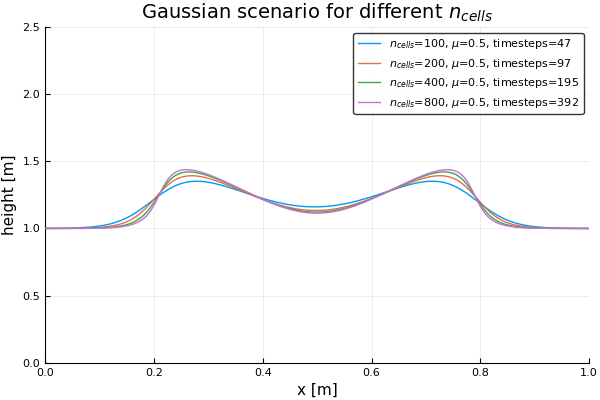
\includegraphics[scale=0.6]{../plots/lxf_gaussian_ncells.png}%
 		\caption{LxF performance relative to $n_{cells}$}\label{fig:lxf_gaussian_ncells}%
 	\end{center}%
\end{figure}

\begin{figure}[h]%
 	\begin{center}%
 		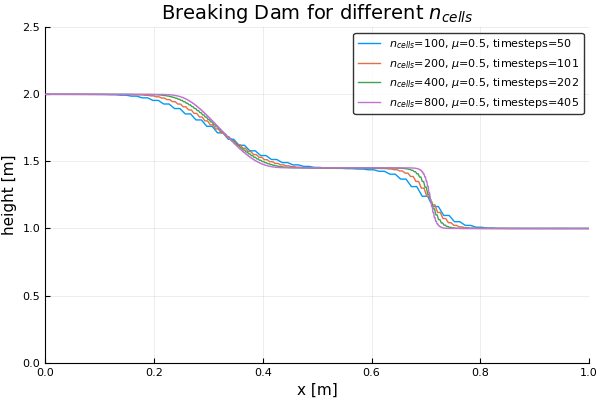
\includegraphics[scale=0.6]{../plots/lxf_breakingdam_ncells.png}%
 		\caption{LxF performance relative to $n_{cells}$}\label{fig:lxf_breakingdam_ncells}%
 	\end{center}%
\end{figure}

\begin{figure}[h]%
 	\begin{center}%
 		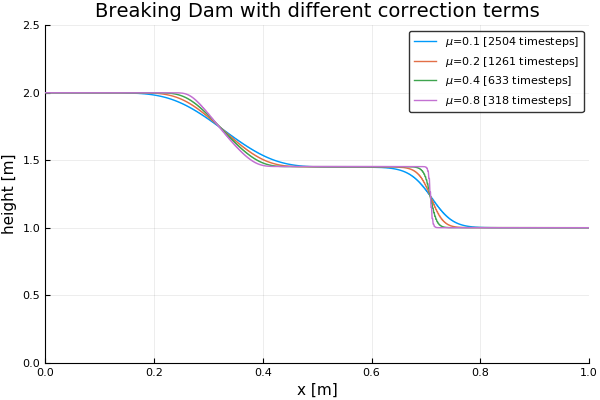
\includegraphics[scale=0.6]{../plots/lxf_breakingdam_mu.png}%
 		\caption{LxF performance relative to $\mu$}\label{fig:lxf_breakingdam_mu}%
 	\end{center}%
\end{figure}

The experiment depicted in Figure~\ref{fig:lxf_gaussian_ncells} is rather intuitive. The Gaussian perturbation propagates symmetrically across the spatial domain. As the spatial discretization is refined, a shock wave gradually emerges from each (previously symmetric) ripple. It should be noted that these shock waves are smeared across tens or hundreds of cells, far more than the finite volume method presumably requires. Furthermore, the crest is reduced and the troughs are filled in: coarsening the mesh increases dissipation.

Applying the same experiment to the breaking dam scenario, as shown in Figure~\ref{fig:lxf_breakingdam_ncells}, yields an additional, unexpected twist. As the mesh becomes coarser, a nonphysical stairstep pattern emerges. This can be directly traced back to the update rule: $Q_i^{n+1}$ depends on $Q_{i+1}^n$ and $Q_{i-1}^n$, but not $Q_{i}^n$. As a result, the odd and even grid cells evolve independently from each other and any disparity between the two oscillates without dampening. Thus the stairstep pattern did not manifest in the Gaussian scenario because the initial condition was smooth. 

The final experiment considers the effect of the timestep correction $\mu$. It uses a fine mesh in order to reduce the dissipation described previously. As defined earlier, $\mu$ is a constant factor which scales down the timestep in order to maintain stability even in the presence of large nonlinearities. However, the behavior shown is remarkably counterintuitive: As the timestep is decreased, the solution becomes more dissipative, and consequently less accurate. When $\mu=1.0$, the shock is crisp and almost vertical; when $\mu=0.1$, the shock is effectively lost. The next section shall explore the cause of this phenomenon by showing how viscous behavior can arise as a result of the numerical method used, rather than the underlying physical system.


\section{Artificial Viscosity}

The key idea behind artificial viscosity is that an approximate solution to a certain problem is oftentimes an exact solution to an approximation of that problem. The trick is to regard simple discretizatons of PDEs as being building blocks which can be assembled into more sophisticated (and correspondingly more approximate) discretizations. One can then map the sophisticated discretization directly back to a modified PDE. In the case of Lax-Friedrichs, the approximation chosen for the flux function is effectively adding a diffusive term to the shallow-water equations. 

Suppose that the `pure' solution to the shallow water equations, $q_t + {f(q)}_x = 0$, corresponds to the naive flux function 

\[F_{i+1/2} = \frac{1}{2} \Big[f(Q_{i+1}) + f(Q_{i})\Big]\] 

even though this is known to be unstable. Similarly, suppose that the `pure' solution to the diffusion equation, $q_t = \beta q_{xx}$, corresponds to the flux function 

\[F_{i+1/2} = -\beta \frac{Q_{i+1} - Q_{i}}{\Delta x}\]

This can be derived by a straightforward finite difference approximation. The Lax-Friedrichs flux function shown previously can be trivially rearranged as: 

\[ F_{i+1/2} = \frac{1}{2} \Big[f(Q_{i}) + f(Q_{i+1})\Big] - \frac{\Delta x}{2\Delta t}\Big[Q_{i+1} - Q_{i}\Big] \]

It is clear that this flux function pattern-matches the discretization of a different PDE:

\[ q_t + f(q)_x = \frac{(\Delta x)^2}{2\Delta t} q_{xx} \]

Thus the Lax-Friedrichs parameter $a = \frac{\Delta x}{\Delta t}$ controls the diffusion coefficient $\beta$ according to 

\[\beta = \frac{(\Delta x)^2}{2\Delta t} = \frac{1}{2} a \Delta x \]

This explains the two results described previously. Firstly, by taking $a$ as constant, and reducing the cell size $\Delta x \to 0$, it is clear that $\beta \to 0$ and the viscous term in the PDE vanishes. Thus the Lax-Friedrichs discretization remains consistent with the pure shallow-water equations.

Secondly, reducing the timestep size $\Delta t$ increases $a$, which then increases $\beta$. This explains the counterintuitive phenomenon where the solution becomes increasingly dissipative, and hence less accurate, as the timestep size is decreased. This then raises the question of whether it is possible to decouple $\beta$ from $\Delta t$ while still maintaining a consistent and stable discretization. The method described in the following section mostly achieves this.


\section{The Local-Lax-Friedrichs Method}

Local-Lax-Friedrichs is a modification which retains the stability benefits of artificial viscosity while decreasing the resulting dissipation. In the basic Lax-Friedrichs, the viscosity parameter $a$ is derived from the CFL condition via $\Delta t$. Although the timestep must be constant in space (local time stepping is not considered), the viscosity may vary. This yields advantages: in regions with shocks or other discontinuities, the presence of viscosity improves numerical stability, and in smooth regions, the lack of viscosity leads to a less dissipative and hence more accurate solution. 


\begin{figure}[t]%
    \begin{center}%
        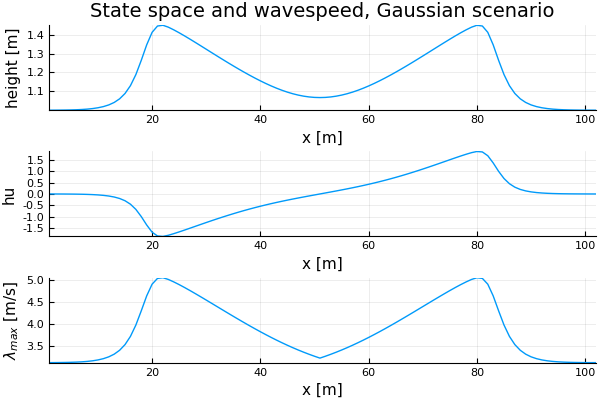
\includegraphics[scale=0.6]{../plots/artificial_viscosity.png}%
        \caption{Wavespeed over the spatial domain}\label{fig:artificial_viscosity}%
    \end{center}%
\end{figure}

\begin{figure}[t]%
    \begin{center}%
        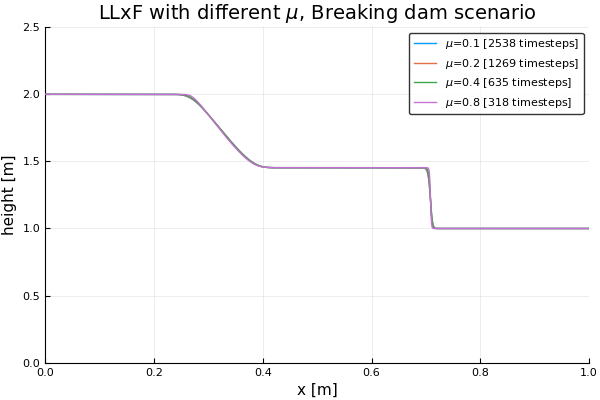
\includegraphics[scale=0.6]{../plots/llxf_breakingdam_mu.png}%
        \caption{Local Lax-Friedrichs, breaking dam scenario. }\label{fig:llxf_breakingdam_mu}%
    \end{center}%
\end{figure}

The viscosity parameter $a$ is taken to be the maximum of the wavespeeds of either neighboring cell. As shown in Figure~\ref{fig:artificial_viscosity}, this exhibits the desired behavior of being large in regions which are discontinuous or evolving quickly, and being small elsewhere. 

\[a_{i-1/2} = \max(\lvert f'(q) \rvert) \ \forall q \in (Q_{i-1}, Q_{i})\]

\begin{equation}
\label{eq:llxf}
F_{i-1/2} = \frac{1}{2}[f(Q_{i-1}) + f(Q_i) - a_{i-1/2}(Q_i - Q_{i-1})]
\end{equation}

From the CFL condition, it is clear that this approach is strictly less viscous than basic Lax-Friedrichs:

\[\lvert f'(q)\rvert \leq \frac{\Delta x}{\Delta t}\]


The Local Lax-Friedrichs method does not entirely break the coupling between dissipation and $\mu$, but it strongly reduces it, as depicted in Figure~\ref{fig:llxf_breakingdam_mu}. This experiment used the exact same parameters as Figure~\ref{fig:lxf_breakingdam_mu}, substituting only the LxF kernel (Eq.~\ref{eq:lxf} with the LLxF kernel (Eq.~\ref{eq:llxf}).

\section{Comparison of LxF vs LLxF}

A final round of experiments were conducted to compare Lax-Friedrichs to Local Lax Friedrichs. These indicate that Local Lax-Friedrichs is decidedly less dissipative and more accurate. Figure~\ref{fig:cmp_breakingdam} shows the results of running LLxF with a middling $\mu=0.4$ against LxF with different $\mu$ for the breaking dam scenario.

At $\mu=0.4$, the LLxF method performs only slightly worse than LxF at $\mu=1.0$. For any given choice of $\mu$, the LLxF reaches a better solution in the same number of timesteps. The quality of the solutions converge as $\mu \to 1.0$. On the other hand, LLxF requires additional work to calculate $a(x)$ for each cell, though the amount is small and linear in the number of cells.

The stairstep oscillations observed in the breaking dam case for LxF are not present for LLxf. This is presumably because the value of $Q_i^n$ enters into the calculation of $Q_i^{n+1}$, albeit rather indirectly, via the max wavespeed $\lambda_{max}$ and then the cell-wise flux $F_{i+1/2}^n$.

\begin{figure}[t]%
    \begin{center}%
        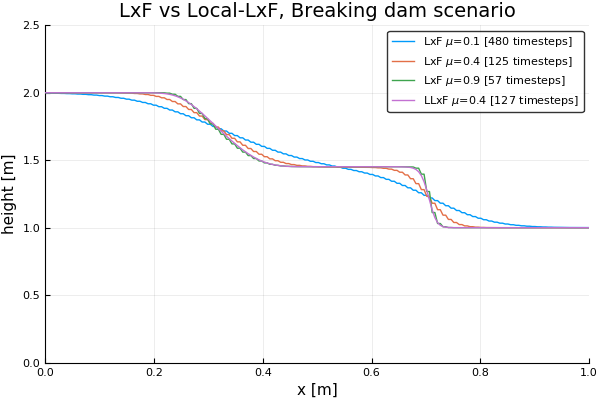
\includegraphics[scale=0.6]{../plots/lxf_llxf_breakingdam.png}%
        \caption{Comparison of Lax-Friedrichs vs Local Lax-Friedrichs, breakin dam scenario}\label{fig:cmp_breakingdam}%
    \end{center}%
\end{figure}

\begin{figure}[t]%
    \begin{center}%
        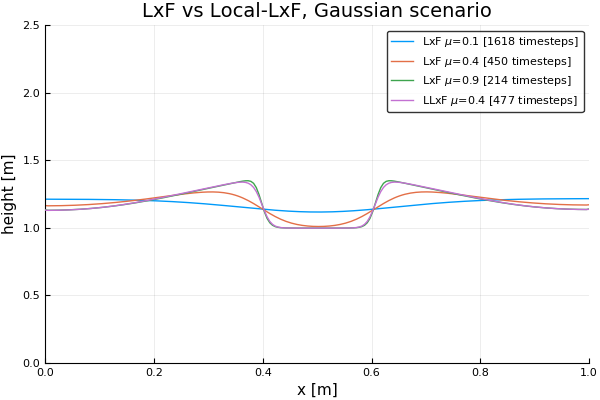
\includegraphics[scale=0.6]{../plots/lxf_llxf_gaussian.png}%
        \caption{Comparison of Lax-Friedrichs vs Local Lax-Friedrichs, gaussian perturbation scenario.}\label{fig:cmp_gaussian}%
    \end{center}%
\end{figure}

\section{Implementation}

This final section describes the design decisions behind the implementation. It is written in Julia, which permits the code to be both notably terse and closely mapped to the theory. The code organization parallels the theoretical development in the preceding sections. 

The first design decision is the choice of data representation. Julia eschews standard object-oriented idioms such as inheritance and encapsulation in favor of a more functional and data-driven approach. Thus the state space $Q$ is a simple mutable structure. The spatial domain $q(x) \forall x$ is defined as a one-dimensional array $QS$ with inner type $Q$. The spatial domain has a ghost cell on either side to enforce boundary conditions, so the physical cell indices range over $[2, n_{cells}+1]$. 

These additional constraints could be expressed within the type system. Firstly, by using \verb!OffsetArray!s, the indices can be cheaply translated to $[1, n_{cells}]$. Secondly, one may parameterize by the number of cells, \verb|QS{ncells}|, e.g. by using \verb|StaticArray|s, ensuring that the array size is known at JIT-compile time. This allows for array-size correctness checks and compiler optimizations. Finally, a custom constructor could encapsulate this and enforce the existence of the ghost cells. These features may prove helpful on larger projects, but were omitted here because they introduce more complexity than they resolve.

The choice of an array-of-structures representation is consistent with the theory, but disregards the fact that $Q$ forms a vector space. This problem is readily resolved thanks to Julia's \emph{multiple dispatch}, where a function is resolved to a method by examining all of the types in the signature, rather than simply the `owning' object.\cite{doi:10.1137/141000671} This means that operations such addition can be extended to custom types in a unified way. Lines 12--26 extend addition and scalar multiplication over the state space type $Q$.

 The general finite volume skeleton (Eq.~\ref{eq:fv}) is given on lines 38--61. The skeleton accepts abstract strategies for flux computations, timestep computations, initial conditions, and boundary conditions. These strategies are implemented as first-class functions rather than as an object heirarchy. Strategies for LxF fluxes (Eq.~\ref{eq:lxf}) and LLxF fluxes (Eq.~\ref{eq:llxf}) are implemented on lines 62--74 and 75--88, respectively. Lines 91--93 demonstrate a higher-order function which acts like a constructor for timestep strategies. Lines 100--102 demonstrate \emph{currying} to convert a three-argument \verb!cfl_dt()! into a two-argument version. Lines 104--112 demonstrate using the method's \emph{closure} to store arbitrary state, in this case the $\Delta t$ calculated during the preceding function call. Finally, lines 147--148 ties everything together to run Lax-Friedrichs on a breaking dam scenario.

% The cell-wise fluxes $F_{i+1/2}, F_{i-1/2}$ are represented slightly differently in the code


\section{Conclusion}

The Lax-Friedrichs method is a simple finite volume technique for solving the shallow water equations. Starting from the fundamentals, this paper built up a reference implementation which leverages features of Julia to achieve terseness and clarity. An abstract finite volume skeleton allows different numerical methods to be swapped in. Two variants were implemented, Lax-Friedrichs and Local Lax-Friedrichs. The former suffers from excessive numerical viscosity, which the latter largely remedies. The causes and consequences of this viscosity were discussed with respect to two model problems, a Gaussian perturbation and a breaking dam. It is the author's hope that this document may serve as a concise guide to students exploring this material in the future. 



%\section*{Acknowledgment}
%\addcontentsline{toc}{section}{Acknowledgment}

% trigger a \newpage just before the given reference
% number - used to balance the columns on the last page
% adjust value as needed - may need to be readjusted if
% the document is modified later
%\IEEEtriggeratref{8}
% The "triggered" command can be changed if desired:
%\IEEEtriggercmd{\enlargethispage{-5in}}

% references section
% NOTE: BibTeX documentation can be easily obtained at:
% http://www.ctan.org/tex-archive/biblio/bibtex/contrib/doc/

% can use a bibliography generated by BibTeX as a .bbl file
% standard IEEE bibliography style from:
% http://www.ctan.org/tex-archive/macros/latex/contrib/supported/IEEEtran/bibtex
\bibliographystyle{IEEEtran}
% argument is your BibTeX string definitions and bibliography database(s)
\bibliography{IEEEabrv,../references}
\newpage
\section{Appendix: Code Listing}
\vspace{1em}
\definecolor{bg}{rgb}{0.95,0.95,0.95}

\begin{myjulia}
# Define precision
const Float = Float64

# Define state space datatype
mutable struct Q
    h :: Float
    hu :: Float
end

# Define spatial domain datatype
QS = Array{Q,1}
\end{myjulia}

\begin{myjulia}
# Make Q a vector space

import Base.+, Base.-, Base.*

function +(lhs::Q, rhs::Q)
    Q(lhs.h + rhs.h, lhs.hu + rhs.hu)
end

function -(lhs::Q, rhs::Q)
    Q(lhs.h - rhs.h, lhs.hu - rhs.hu)
end

function *(a::Real, q::Q)
    Q(a*q.h, a*q.hu)
end
\end{myjulia}

\begin{myjulia}
"Shallow-water point-wise flux"
function f(q :: Q)
    Q(q.hu, q.hu^2/q.h + 0.5*G*q.h^2)
end

"Shallow-water point-wise max wave speed"
function wavespeed(q :: Q)
    u = q.hu / q.h
    c = sqrt(G * q.h)
    max(abs(u-c), abs(u+c))
end

\end{myjulia}

\begin{myjulia}

"Finite volume skeleton"
function run(stoptime::Real, ncells::Int, choose_dt,
             compute_fluxes!, apply_bcs!, apply_ics)

    qs = apply_ics(ncells)
    Fl = QS(ncells+2)
    Fr = QS(ncells+2)

    currenttime = 0
    timesteps = 0
    dx = Float(1000.0/ncells)
    
    while currenttime < stoptime
        apply_bcs!(qs)
        dt = choose_dt(qs, dx)
        compute_fluxes!(qs, Fl, Fr, ncells, dx, dt)
        for x = 2:ncells+1
            qs[x] -= dt/dx * (Fr[x] + Fl[x-1])
        end
        currenttime += dt
        timesteps += 1
    end
    return (qs, currenttime, timesteps)
end
\end{myjulia}
\begin{myjulia}

"Lax-Friedrichs kernel"
function lxf!(qs::QS, Fl::QS, Fr::QS, 
              ncells::Int, dx::Float, dt::Float)
    
    a = dx/dt
    for x = 2:ncells+2
        ql,qr = qs[x-1], qs[x]
        fl,fr = f(ql), f(qr)        

        Fr[x-1] = 0.5*((fr-fl) - a*(qr - ql))
        Fl[x-1] = 0.5*((fr-fl) + a*(qr - ql))
    end
end

\end{myjulia}
\newpage
\begin{myjulia}

"Local Lax-Friedrichs kernel"
function llxf!(qs::QS, Fl::QS, Fr::QS, 
               ncells::Int, dx::Float, dt::Float)
    
    for x = 2:ncells+2
        ql,qr = qs[x-1], qs[x]
        fl,fr = f(ql), f(qr)

        a = max(wavespeed(ql), wavespeed(qr))

        Fr[x-1] = 0.5*((fr-fl) - a*(qr-ql))
        Fl[x-1] = 0.5*((fr-fl) + a*(qr-ql))
    end
end
\end{myjulia}
\begin{myjulia}
# Timestepping strategies: (QS, dx) -> dt

function make_const_dt(dt::Float)
    return (qs, dx) -> dt
end

function cfl_dt(qs::QS, dx::Real, mu::Real)
    lambda = map(wavespeed,qs) |> maximum
    return Float(dx / lambda * mu)
end

function make_cfl_dt(mu::Real)
    return (qs, dx) -> cfl_dt(qs, dx, mu)
end

function make_lagging_dt(dt0::Real, mu::Real)
    dt = dt0
    function lagging_dt(qs, dx)
        result = dt
        dt = cfl_dt(qs, dx, mu)
        return result
    end
    return lagging_dt
end
\end{myjulia}

\begin{myjulia}
# Initial conditions: ncells -> QS

function gaussian_ics(ncells::Int)
    qs = QS(ncells+2)
    mid = ncells / 2.0 + 1
    for x = 1:ncells+2
        pos_rel = (mid-x) / (ncells/10.0)
        qs[x] = Q(exp(-pos_rel^2) + 1, 0.0)
    end
    return qs
end

function breakingdam_ics(ncells::Int)
    [x < ncells/2 ? Q(2,0) : Q(1,0) for x in 1:ncells+2]
end
\end{myjulia}

\begin{myjulia}
# Boundary conditions: QS -> nothing 

function outflow_bcs!(qs::QS)
    qs[1] = qs[2]
    qs[end] = qs[end-1]
end

function periodic_bcs!(qs::QS)
    qs[1] = qs[end-1]
    qs[end] = qs[2]
end

function reflecting_bcs!(qs::QS)
    qs[1].h = qs[2].h
    qs[1].hu = -qs[2].hu
    qs[end].h = qs[end-1].h
    qs[end].hu = -qs[end-1].hu
end
\end{myjulia}

\begin{myjulia}

# Sample experiment run
qs,t,ts = run(50, 1000, make_cfl_dt(0.5), 
              lxf!, outflow_bcs!, breakingdam_ics)

\end{myjulia}


%
% <OR> manually copy in the resultant .bbl file
% set second argument of \begin to the number of references
% (used to reserve space for the reference number labels box)
%\begin{thebibliography}{1}
%
%\bibitem{ref:kopka}
%H.~Kopka and P.~W. Daly, \emph{A Guide to {\LaTeX}}, 3rd~ed.\hskip 1em plus
%  0.5em minus 0.4em\relax Harlow, England: Addison-Wesley, 1999.
%
%\end{thebibliography}

\end{document}


